\section{Test Cases}
\label{ch2:sec:test_cases}
The IEEE Power and Energy Society (IEEE-PES) provides several test cases. The present validation examines and tests the following: 

\subsection{IEEE 33 Node Test Feeder}
Figure \ref{ch2:fig:33bus} shows the IEEE 33 node test feeder topology and Table \ref{ch2:tab:dn_data} summaries its parameters. 
\begin{figure}
    \centering
    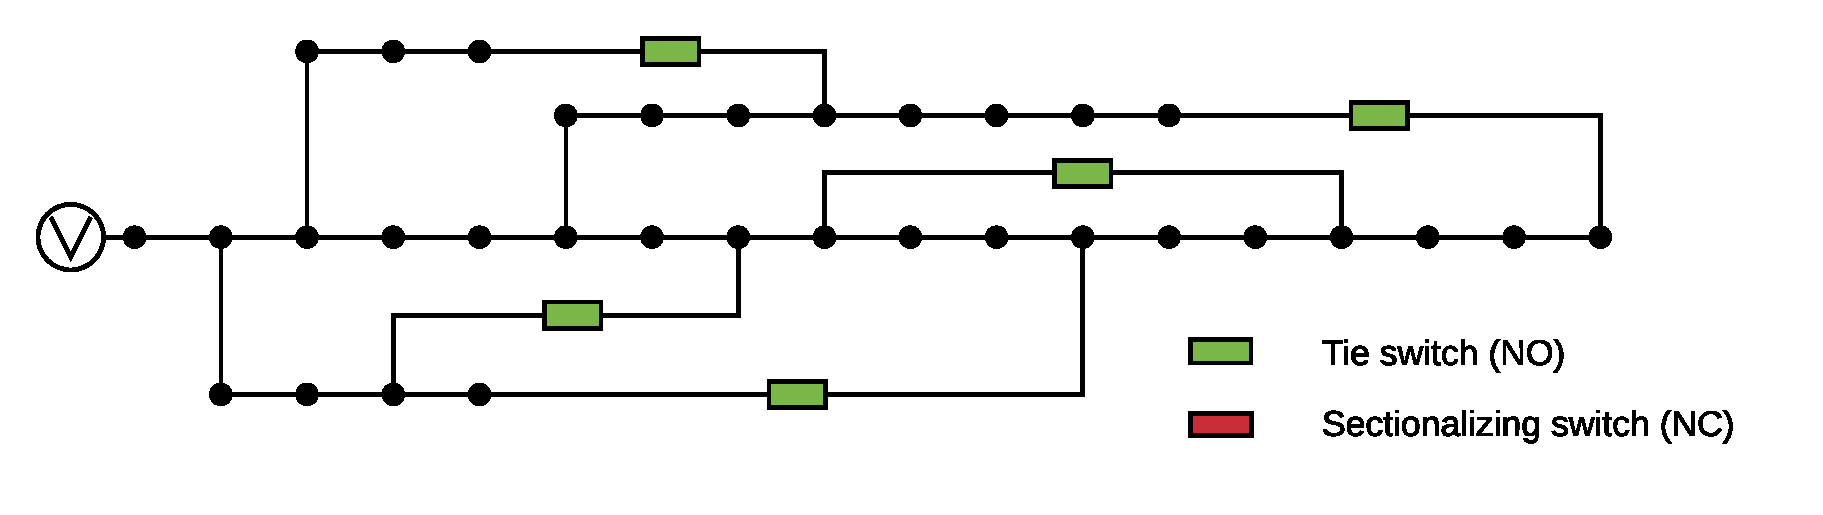
\includegraphics[scale=0.4]{_chapter2/fig/33bus_tc.pdf}
    \caption{IEEE 33 Node Test Feeder from \cite{Landeros2019}}
    \label{ch2:fig:33bus}
\end{figure}

\begin{table}
\centering
\caption{IEEE test feeders data}
\label{ch2:tab:dn_data}
    \begin{tabular}{lcc}
    \hline
    \textbf{DN Elment}         & \textbf{\begin{tabular}[c]{@{}c@{}}33 Node\\ Test Feeder\end{tabular}} & \textbf{\begin{tabular}[c]{@{}c@{}}123 Node \\ Test Feeder\end{tabular}} \\ \hline
    \textit{\textbf{Lines}}    & 32                                                                     & 117                                                                      \\
    \textit{\textbf{Switches}} & 2 - 5                                                                      & 5 - 15                                                                     \\
    \textit{\textbf{Loads}}    & 32                                                                     & 91                                                                      
    \end{tabular}
    \end{table}

\subsection{IEEE 123 Node Test Feeder}

This system is modified to observe the behavior of the Service Restoration Algorithm and to compare 
its performance according to the number of switches. For this reason, they have tested ten variants 
of this test feeder. Each modification increases the number of switches by one, where the minimum is 
five switches and the maximum is fifteen.

Figure \ref{ch2:fig:123bus} shows the IEEE 123 node test feeder topology with 10 switches and 
Table \ref{ch2:tab:dn_data} summaries its parameters. 
\begin{figure}
    \centering
    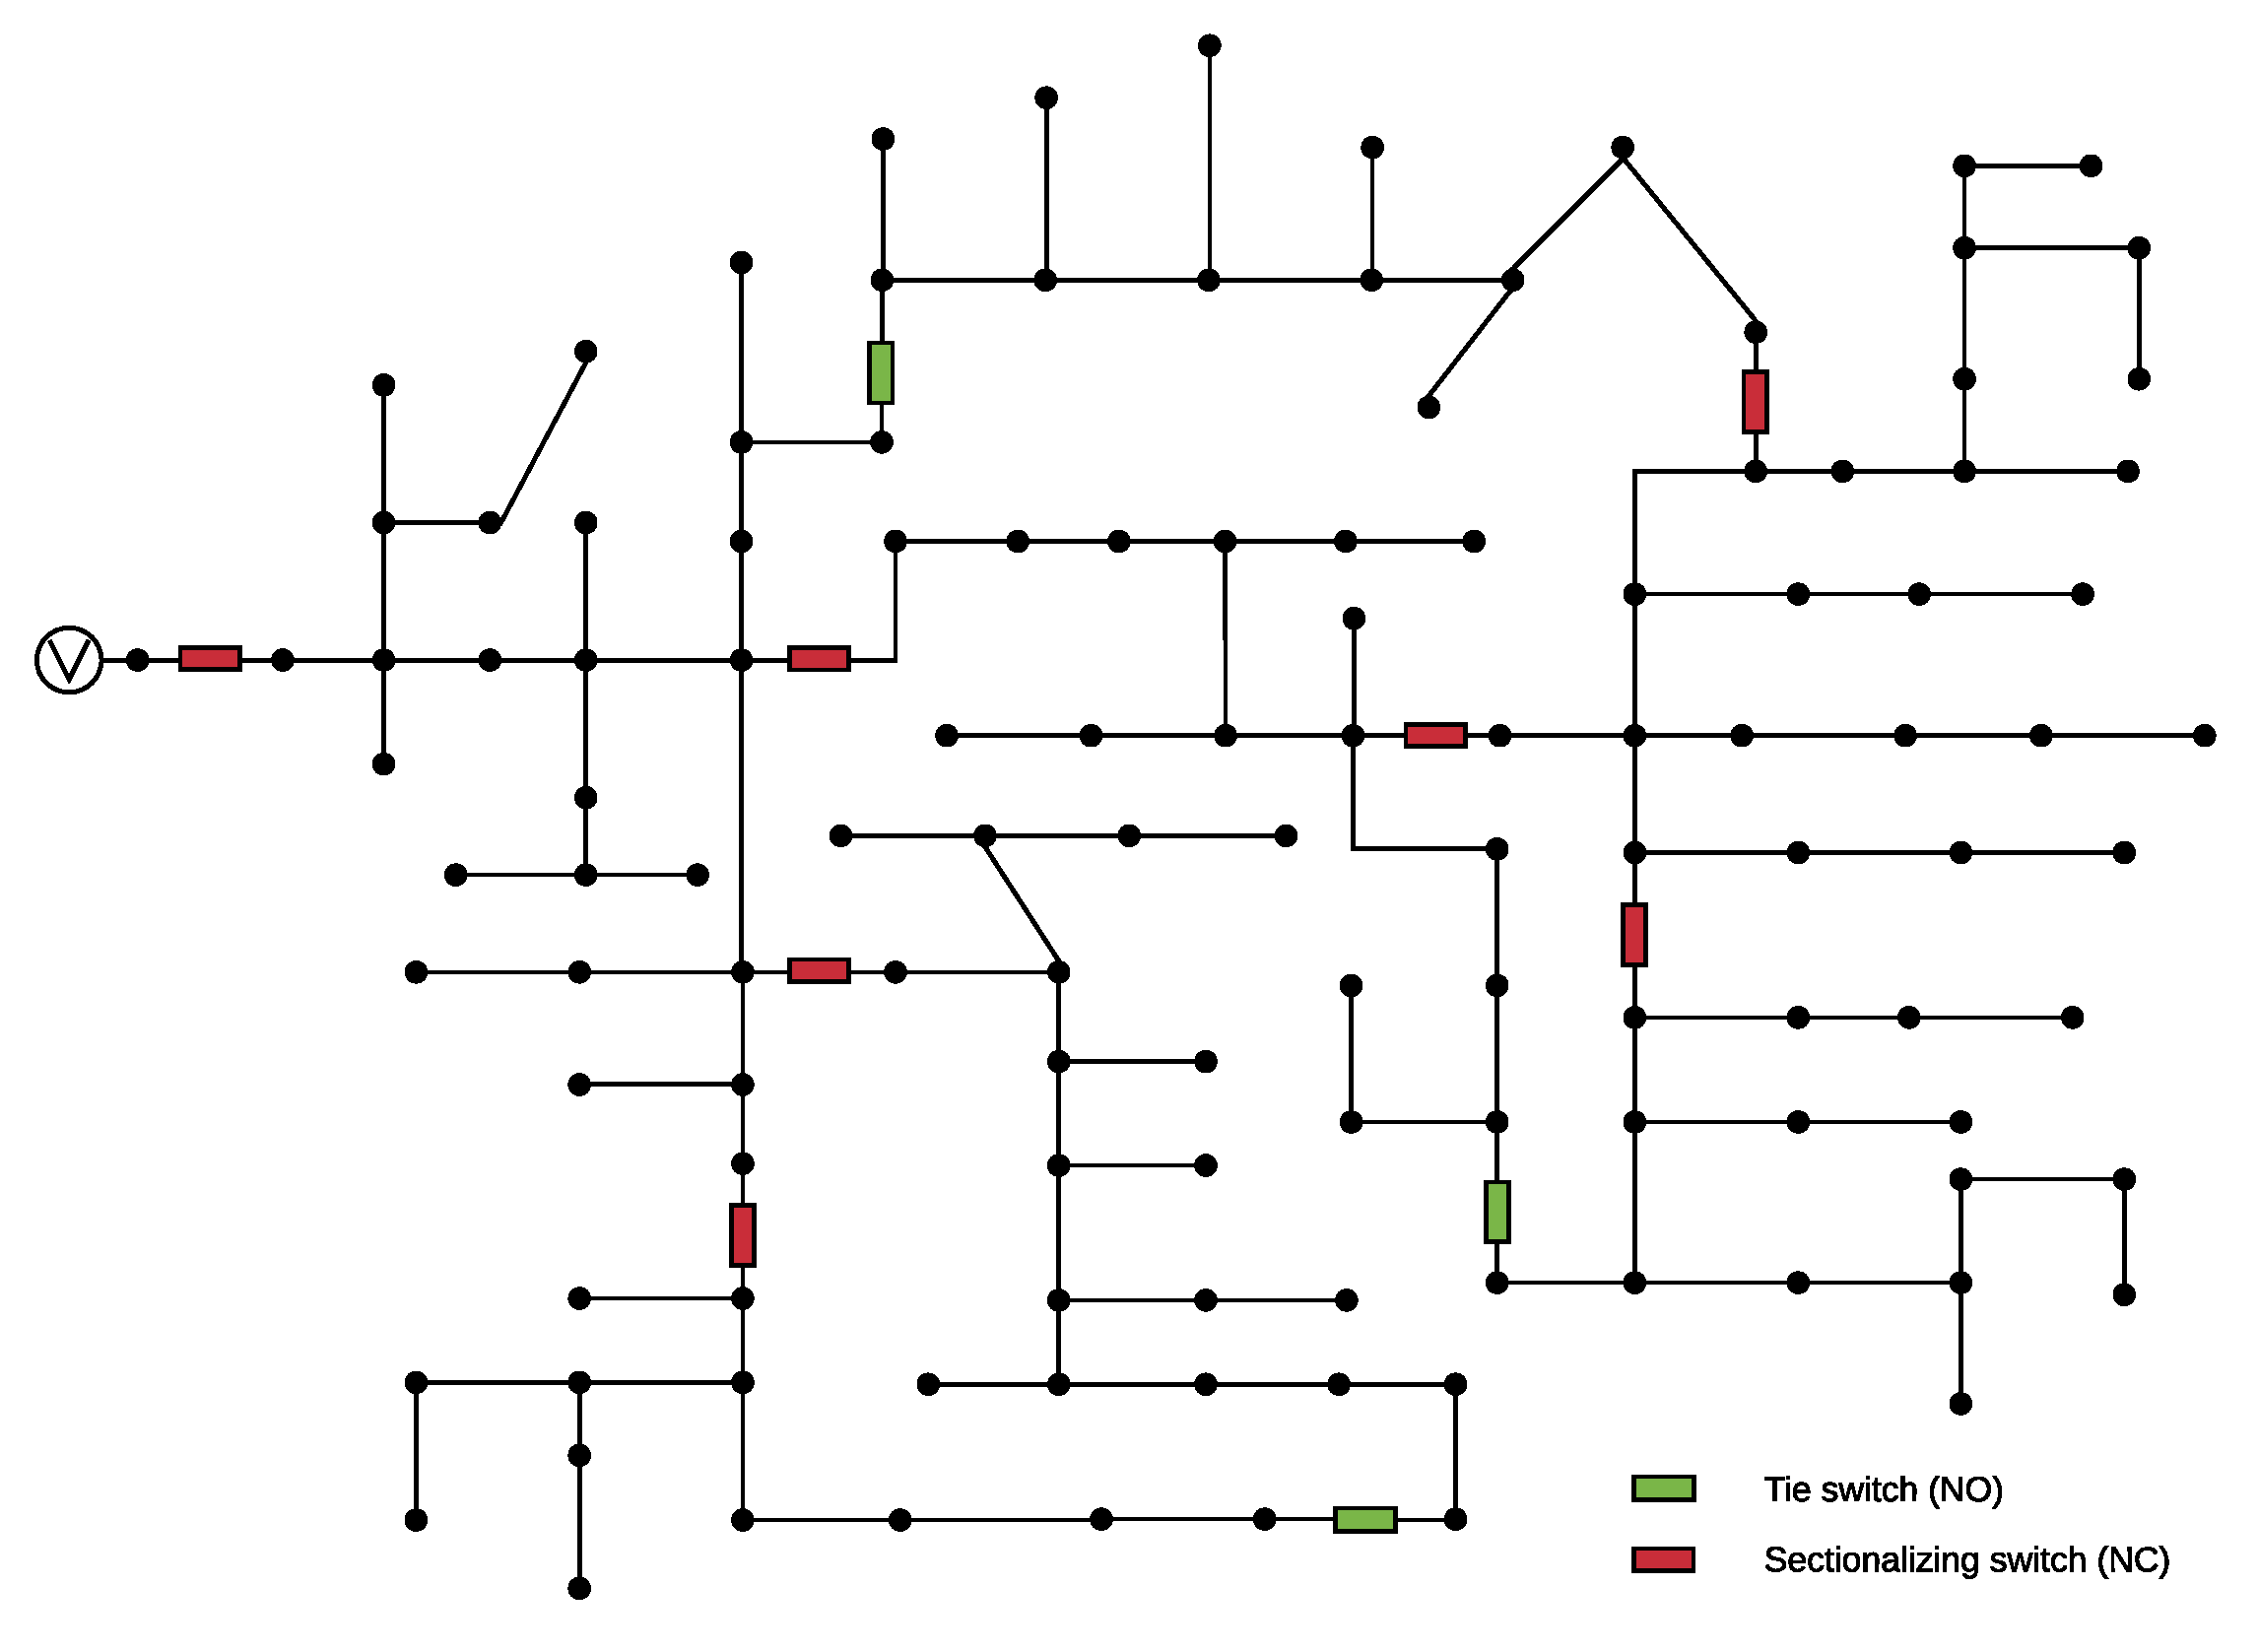
\includegraphics[scale=0.35]{_chapter2/fig/123iee_tc.pdf}
    \caption{IEEE 123 Node Test Feeder}
    \label{ch2:fig:123bus}
\end{figure}

%\subsection{IEEE 8500 Node Test Feeder}
%Figure \ref{ch2:fig:8500bus} shows the IEEE 123 node test feeder topology and Table \ref{ch2:tab:dn_data} summaries its
%parameters. This system is modified by reducing the number of switches to 25, due to computational capacities. 

%\begin{figure}
    \centering
    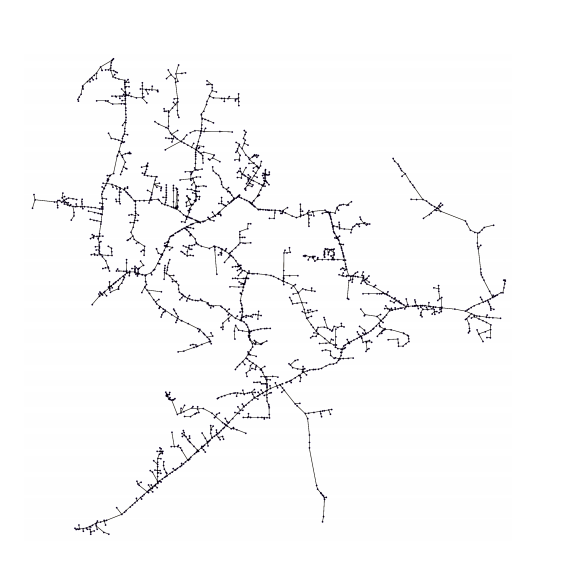
\includegraphics[scale=0.5]{_chapter2/fig/ieee8500.png}
    \caption{IEEE 8500 Node Test Feeder}
    \label{ch2:fig:8500bus}
\end{figure}

